\section{Installation of Asterisk}	\label{sec:run-asterisk}
	To install Asterisk same as this project authors, please follow below instructions: (\textbf{Note:} Here author installing Asterisk from source code. You can also follow the installation video from \href{https://www.youtube.com/watch?v=52sEPVPV9JE&list=PLruX0IBTg1G4Auvo5YhoJKgskmMP7b8bJ&index=4&ab_channel=InnovateAsterisk}{InnovationAsterisk})
	
	\subsection{Asterisk Installation from the Source Code}
		\begin{itemize}[leftmargin=1.7cm]
			\item[\textbf{Step 1:}] Type command ``{\fontfamily{cmtt}\selectfont{wget http://downloads.asterisk.org/pub/telephony/asterisk/asterisk-18-curren\\t.tar.gz}}''\\
				\begin{minipage}{\textwidth}
					\vspace{2mm}
					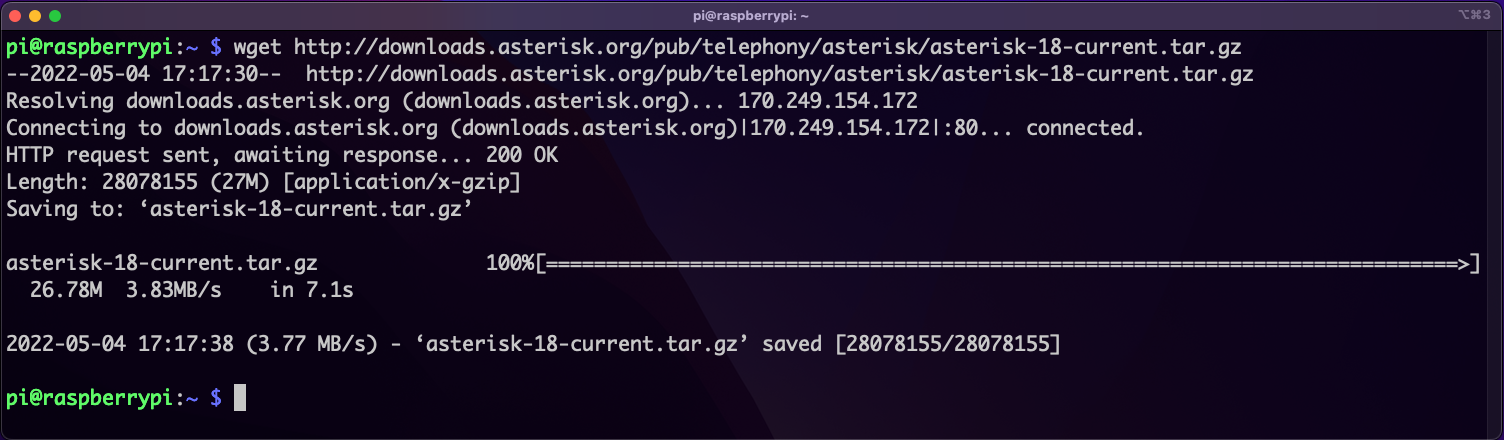
\includegraphics[scale=0.3]{Images/raspberry_pi/asterisk_install/wget.png}
					\vspace{2mm}
				\end{minipage}
			
			\item[\textbf{Step 2:}] Type command ``{\fontfamily{cmtt}\selectfont{sudo apt-get update}}''
			\item[\textbf{Step 3:}] Type command ``{\fontfamily{cmtt}\selectfont{sudo apt-get upgrade}}''
			\item[\textbf{Step 4:}] Type command ``{\fontfamily{cmtt}\selectfont{sudo apt-get install ntp}}''
			\item[\textbf{Step 5:}] Type command ``{\fontfamily{cmtt}\selectfont{sudo apt-get install speex speex* libspeex-dev libspeexdsp-dev}}''
			\item[\textbf{Step 6:}] Type command ``{\fontfamily{cmtt}\selectfont{sudo apt-get install libspeex-dev libspeexdsp-dev speex speex-doc}}''
			\item[\textbf{Step 7:}] Type command ``{\fontfamily{cmtt}\selectfont{sudo apt-get install xmlstarlet libopus-dev libopusfile-dev}}'' <-- (\textbf{NOTE:} This optional if you don't want browser-base telephony, here author did not do this)
			
			\item[\textbf{Step 8:}] Type command ``{\fontfamily{cmtt}\selectfont{tar -xvf asterisk-18-current.tar.gz}}'' <-- This command will extract all the source file into folder called ``asterisk-18.x.x'' (\textbf{Note:} here `x' could be any number based of current relese/download)
			
			\item[\textbf{Step 9:}] Type command ``{\fontfamily{cmtt}\selectfont{cd asterisk-18.x.x}}'' <-- (\textbf{Note:} here `x' could be any number based of current relese/download)
			
			\item[\textbf{Step 10:}] Type command ``{\fontfamily{cmtt}\selectfont{sudo contrib/scripts/install\_prereq install}}'' <-- This will check all the prerequisites of Asterisk. This command will ask few promps to set configurations
					\begin{enumerate}
						\item Telephone code : Type ``{\fontfamily{cmtt}\selectfont{1}}'' for US
					\end{enumerate}
			\item[\textbf{Step 11:}] Type command ``{\fontfamily{cmtt}\selectfont{sudo ./configure --libdir=/usr/lib --with-pjproject-bundled}}''
			
			\item[\textbf{Step 12:}] Type command ``{\fontfamily{cmtt}\selectfont{sudo make menuselect}}'' <-- Please watch this \href{https://www.youtube.com/watch?v=52sEPVPV9JE&list=PLruX0IBTg1G4Auvo5YhoJKgskmMP7b8bJ&index=4&ab_channel=InnovateAsterisk}{video}) from InnovateAsterisk for more details.

			\item[\textbf{Step 13:}] Type command ``{\fontfamily{cmtt}\selectfont{sudo make}}''
			\item[\textbf{Step 14:}] Type command ``{\fontfamily{cmtt}\selectfont{sudo make install}}''
			\item[\textbf{Step 15:}] Type command ``{\fontfamily{cmtt}\selectfont{sudo make samples}}'' <-- This will create all default Asterisk configuration files\\\\
			\danger\textbf{NOTE:} \textbf{Step 16-17} is only required if you haven't downloaded ``IoT\_RaspberryPi'' GitHub repository from \href{https://github.com/TrupeshKumarPatel/IoT_RaspberryPi}{here}  \danger\\
			\item[\textbf{Step 16\danger:}] Type command ``{\fontfamily{cmtt}\selectfont{cd ~}}''
			\item[\textbf{Step 17\danger:}] Type command ``{\fontfamily{cmtt}\selectfont{git clone https://github.com/TrupeshKumarPatel/IoT\_RaspberryPi.git}}''\\
				\begin{minipage}{\textwidth}
					\vspace{2mm}
					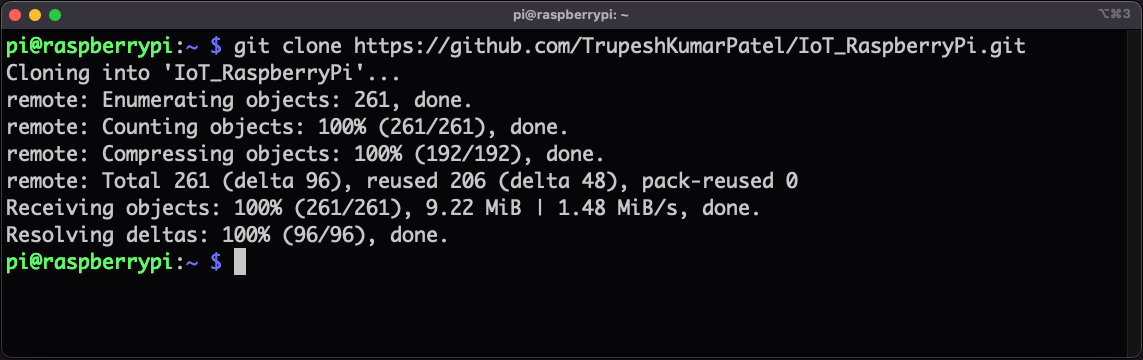
\includegraphics[scale=0.35]{Images/raspberry_pi/eduroam_config/clone_git.png}
					\vspace{2mm}
				\end{minipage}
			\item[\textbf{Step 18:}] Types command ``{\fontfamily{cmtt}\selectfont{sudo cp -R ~/IoT\_RaspberryPi/source\_code/asterisk\_config/* /etc/asterisk/}}''
		\end{itemize}

\pagebreak
\section{Command of Asterisk}	\label{sec:command-asterisk}
	Now, after following instruction from \hyperref[sec:run-asterisk]{Section \ref{sec:run-asterisk}}, you should be able to run asterisk commands.
	\begin{itemize}
		\item To check the status of Asterisk\\
		Type command ``{\fontfamily{cmtt}\selectfont{sudo service asterisk status}}''
		\item To start the Asterisk\\
		Type command ``{\fontfamily{cmtt}\selectfont{sudo service asterisk start}}''
		\item To restart the Asterisk\\
		Type command ``{\fontfamily{cmtt}\selectfont{sudo service asterisk restart}}''
		\item To stop the Asterisk\\
		Type command ``{\fontfamily{cmtt}\selectfont{sudo service asterisk stop}}''
		\item To access CLI of the Asterisk\\
		Type command ``{\fontfamily{cmtt}\selectfont{sudo asterisk -r}}''\\
			\begin{minipage}{\textwidth}
				\vspace{2mm}
				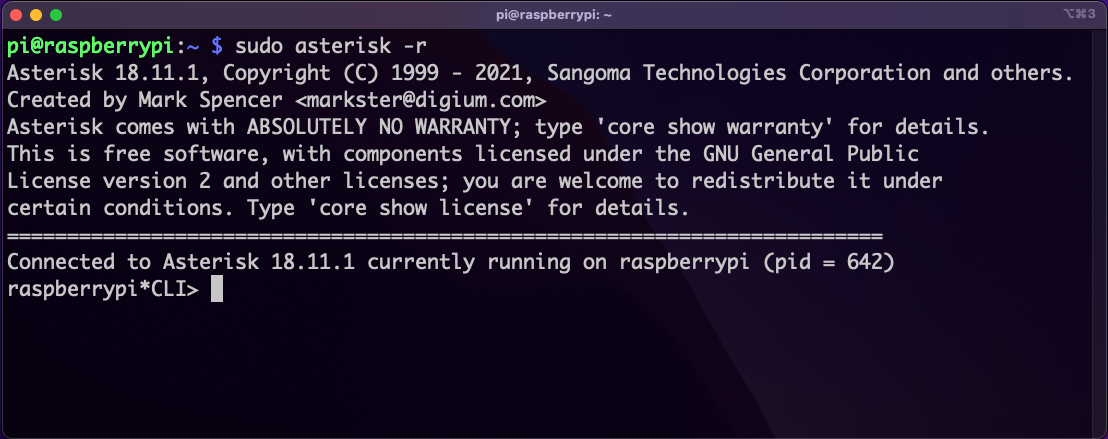
\includegraphics[scale=0.35]{Images/raspberry_pi/asterisk_install/CLI.png}
				\vspace{2mm}
			\end{minipage}
		\item To see all peers\\
		Type command ``{\fontfamily{cmtt}\selectfont{sip show peers}}''\\
			\begin{minipage}{\textwidth}
				\vspace{2mm}
				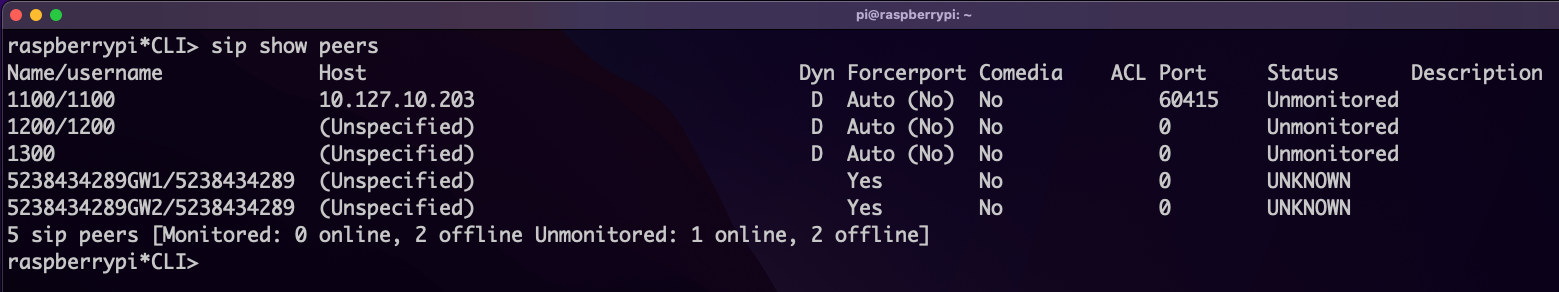
\includegraphics[scale=0.3]{Images/raspberry_pi/asterisk_install/show_peers.png}
				\vspace{2mm}
			\end{minipage}
		\item To see all users\\
		Type command ``{\fontfamily{cmtt}\selectfont{sip show users}}''\\
		\begin{minipage}{\textwidth}
			\vspace{2mm}
			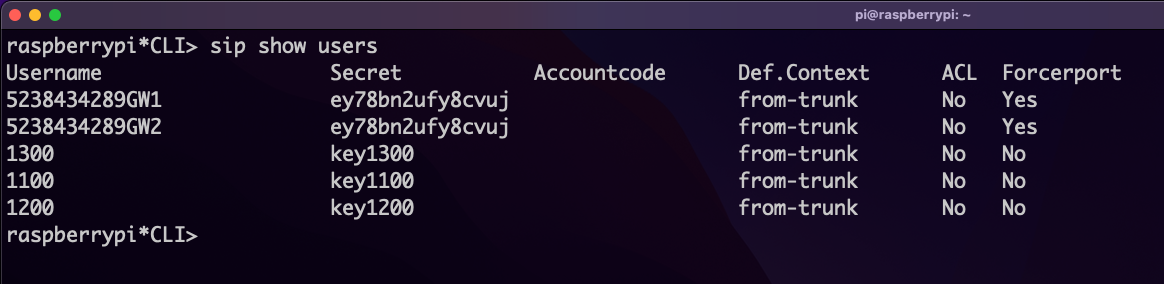
\includegraphics[scale=0.3]{Images/raspberry_pi/asterisk_install/show_users.png}
			\vspace{2mm}
		\end{minipage}
	\end{itemize}
	
	There are many Asterisk commands are available to it's documet \href{https://www.voip-info.org/asterisk-cli/}{here}, use it as you need.